\documentclass[10pt,a4paper,uplatex,dvipdfmx]{jsarticle}
\usepackage{bm}
\usepackage{graphicx}
\usepackage[truedimen,left=25truemm,right=25truemm,top=25truemm,bottom=25truemm]{geometry}
\usepackage{array}
\usepackage{titlesec}
\usepackage{jpdoc}
%\usepackage{tree}
\usepackage[nofiglist,nomarkers]{endfloat}

\renewcommand{\figurename}{別添}
\newcommand{\figref}[1]{別添\ref{#1}}

\titleformat*{\section}{\large\bfseries}
\def\title{組織規程}

\begin{document}
	\newpage
{\centering \Large\bf \title  \vskip 0em}
\vskip 2em

\subsection{総則}
\article{目的}
本規程は、定款に定めるもののほか、株式会社RICOS (以下、「当会社」とする) の組織並びに業務分掌に関する基本事項を明確に定め、業務の効率的かつ組織的、有機的な運営・遂行を図ることを目的とする。
%株主総会及び代表取締役は定款に記載済のため、それ以外について記述

\article{解釈上の疑義}
本規程の解釈に疑義を生じたときは、取締役会の審議 (取締役会設置会社でない場合には取締役の決定) を経て、代表取締役がこれを裁定する。

\subsection{組織構成}
\article{組織運用の原則}
組織の運用にあたっては、役員及び従業員は、定められた基本的な業務を忠実に遂行するとともに、相互に関連のある業務について重複又は間隙を生ぜしめることなく、関係各部署と十分協調し、その活動が効率的に行われるよう、進んで調整を図らなければならない。

\article{組織単位}
当会社の組織単位は、本部、部とする。ただし、必要に応じてその他の組織単位を置くことができることとする。

\article{経営会議}
取締役会決議事項以外の重要事項につき、審議並びに決定を行う機関として、経営会議を設置する。経営会議は「経営会議運営規程」により運営する。

\article{本部長、部長}
本部に本部長、部に部長を置く。
\term 本部長、部長は、代表取締役の命を受けて当該分掌業務を統括し、部所属員を指揮監督して、その業務の発展、伸長をはかると共にその結果について責任を負う。

\article{その他の組織体}
会社の業務を円滑に遂行するため必要ある場合には、プロジェクトチーム、タスクフォース、委員会、会議などの臨時的組織体を設置することができるものとする。その目的、責任者、組織、形態及び運営方法などについてはその都度定めることとする。

\article{職務権限}
職務権限については、別に定める「職務権限規程」によるものとする。

\article{組織図}
当会社の組織図は、別添のとおりとする。

\subsection{各本部における業務分掌}
\article{共通業務分掌}
各部署が、協調して遂行すべき共通業務分掌は、次のとおりとする。
\begin{enumerate}
	\item 経営方針に基づく各部事業計画の立案及び遂行、並びに所管各部署計画の調整及び管理
	\item 各部署予算案の編成及び統制
	\item 各部署の人事管理及び部署内教育、並びに研修計画の立案及び実施
	\item 所管業務に関する資料及び文書の作成、整理及び保管
	\item 所管業務の業務改善及び効率化促進の検討立案
	\item その他特に命じられた業務
\end{enumerate}
\term 他の部署と関連する分掌事項についてはその部署と協議し、他の部署の分掌事項に関しても、所属長の命により協調して支援、補助をするものとする。

\article{管理本部}
管理本部には、人事総務部及び財務経理部を置く。
\term 人事総務部の業務分掌は、次のとおりとする。
\begin{enumerate}
	\item 人事に関すること
	\item 労務管理に関すること
	\item 総務に関すること
	\item 法務に関すること
	\item 競争的資金(公的研究費等)に係る物品役務発注・運営・管理に関すること
	\item その他上記に類する業務    
\end{enumerate}

\term 財務経理部の業務分掌は、次のとおりとする。
\begin{enumerate}
	\item 財務に関すること
	\item 経理に関すること
	\item 経営企画に関すること
	\item 内部統制に関すること
	\item 社内外向け広報活動及びIR活動に関すること
	\item その他上記に類する業務
\end{enumerate}

\article{研究本部}
研究本部には、基盤研究部及び基盤開発部を置く。
\term 基盤研究部の業務分掌は、次のとおりとする。
\begin{enumerate}
	\item 研究計画及び研究予算等に基づき研究活動を行うこと
	\item 法人が開催する研究会・ワークショップ等の企画、実施及び運営に関すること
	\item 研究業績評価等に関すること
	\item 研究成果等の発信、広報活動に関すること
	\item 競争的資金(公的研究費等)に関すること
	\item 研究活動において必要となる調査・その他外部委託契約に関すること
	\item その他上記に類する業務
\end{enumerate}

\term 基盤開発部の業務分掌は、次のとおりとする。
\begin{enumerate}
	\item 研究成果を事業化するための基礎技術の開発に関すること
	\item 基盤技術の開発計画及び開発予算等に基づき開発活動を行うこと
	\item 基盤開発活動において必要となる調査・その他外部委託契約に関すること
	\item その他上記に類する業務
\end{enumerate}

\article{開発本部}
開発本部には、応用開発部を置く。
\term 応用開発部の業務分掌は、次のとおりとする。
\begin{enumerate}
	\item 基盤開発部で開発・事業化された製品の応用技術の開発に関すること
	\item 応用技術の開発計画及び開発予算等に基づき開発活動を行うこと
	\item 応用開発活動において必要となる調査・その他外部委託契約に関すること
	\item その他上記に類する業務
\end{enumerate}

\article{営業本部}
営業本部には、営業部を置く。
\term 営業部の業務分掌は、次のとおりとする。
\begin{enumerate}
	\item 営業計画及び営業予算等に基づき営業活動を行うこと
	\item 事業に関する新規顧客・既存顧客への営業活動及び広報活動に関すること
	\item 営業活動において必要となる取引先の動向把握・市場情報の調査、その他外部委託契約に関すること
	\item その他上記に類する業務
\end{enumerate}

\vspace{1cm}
\subparagraph{附則}本規程の改廃は、「規程類管理規程」に定める手続きによるものとする。
\subparagraph{附則}本規程は、令和2年7月1日から施行する。
\subparagraph{附則}本規程の改正は、令和4年8月15日から施行する。 
\subparagraph{附則}本規程の改正は、令和5年11月1日から施行する。 

\clearpage

\begin{figure}[h]
\centering
	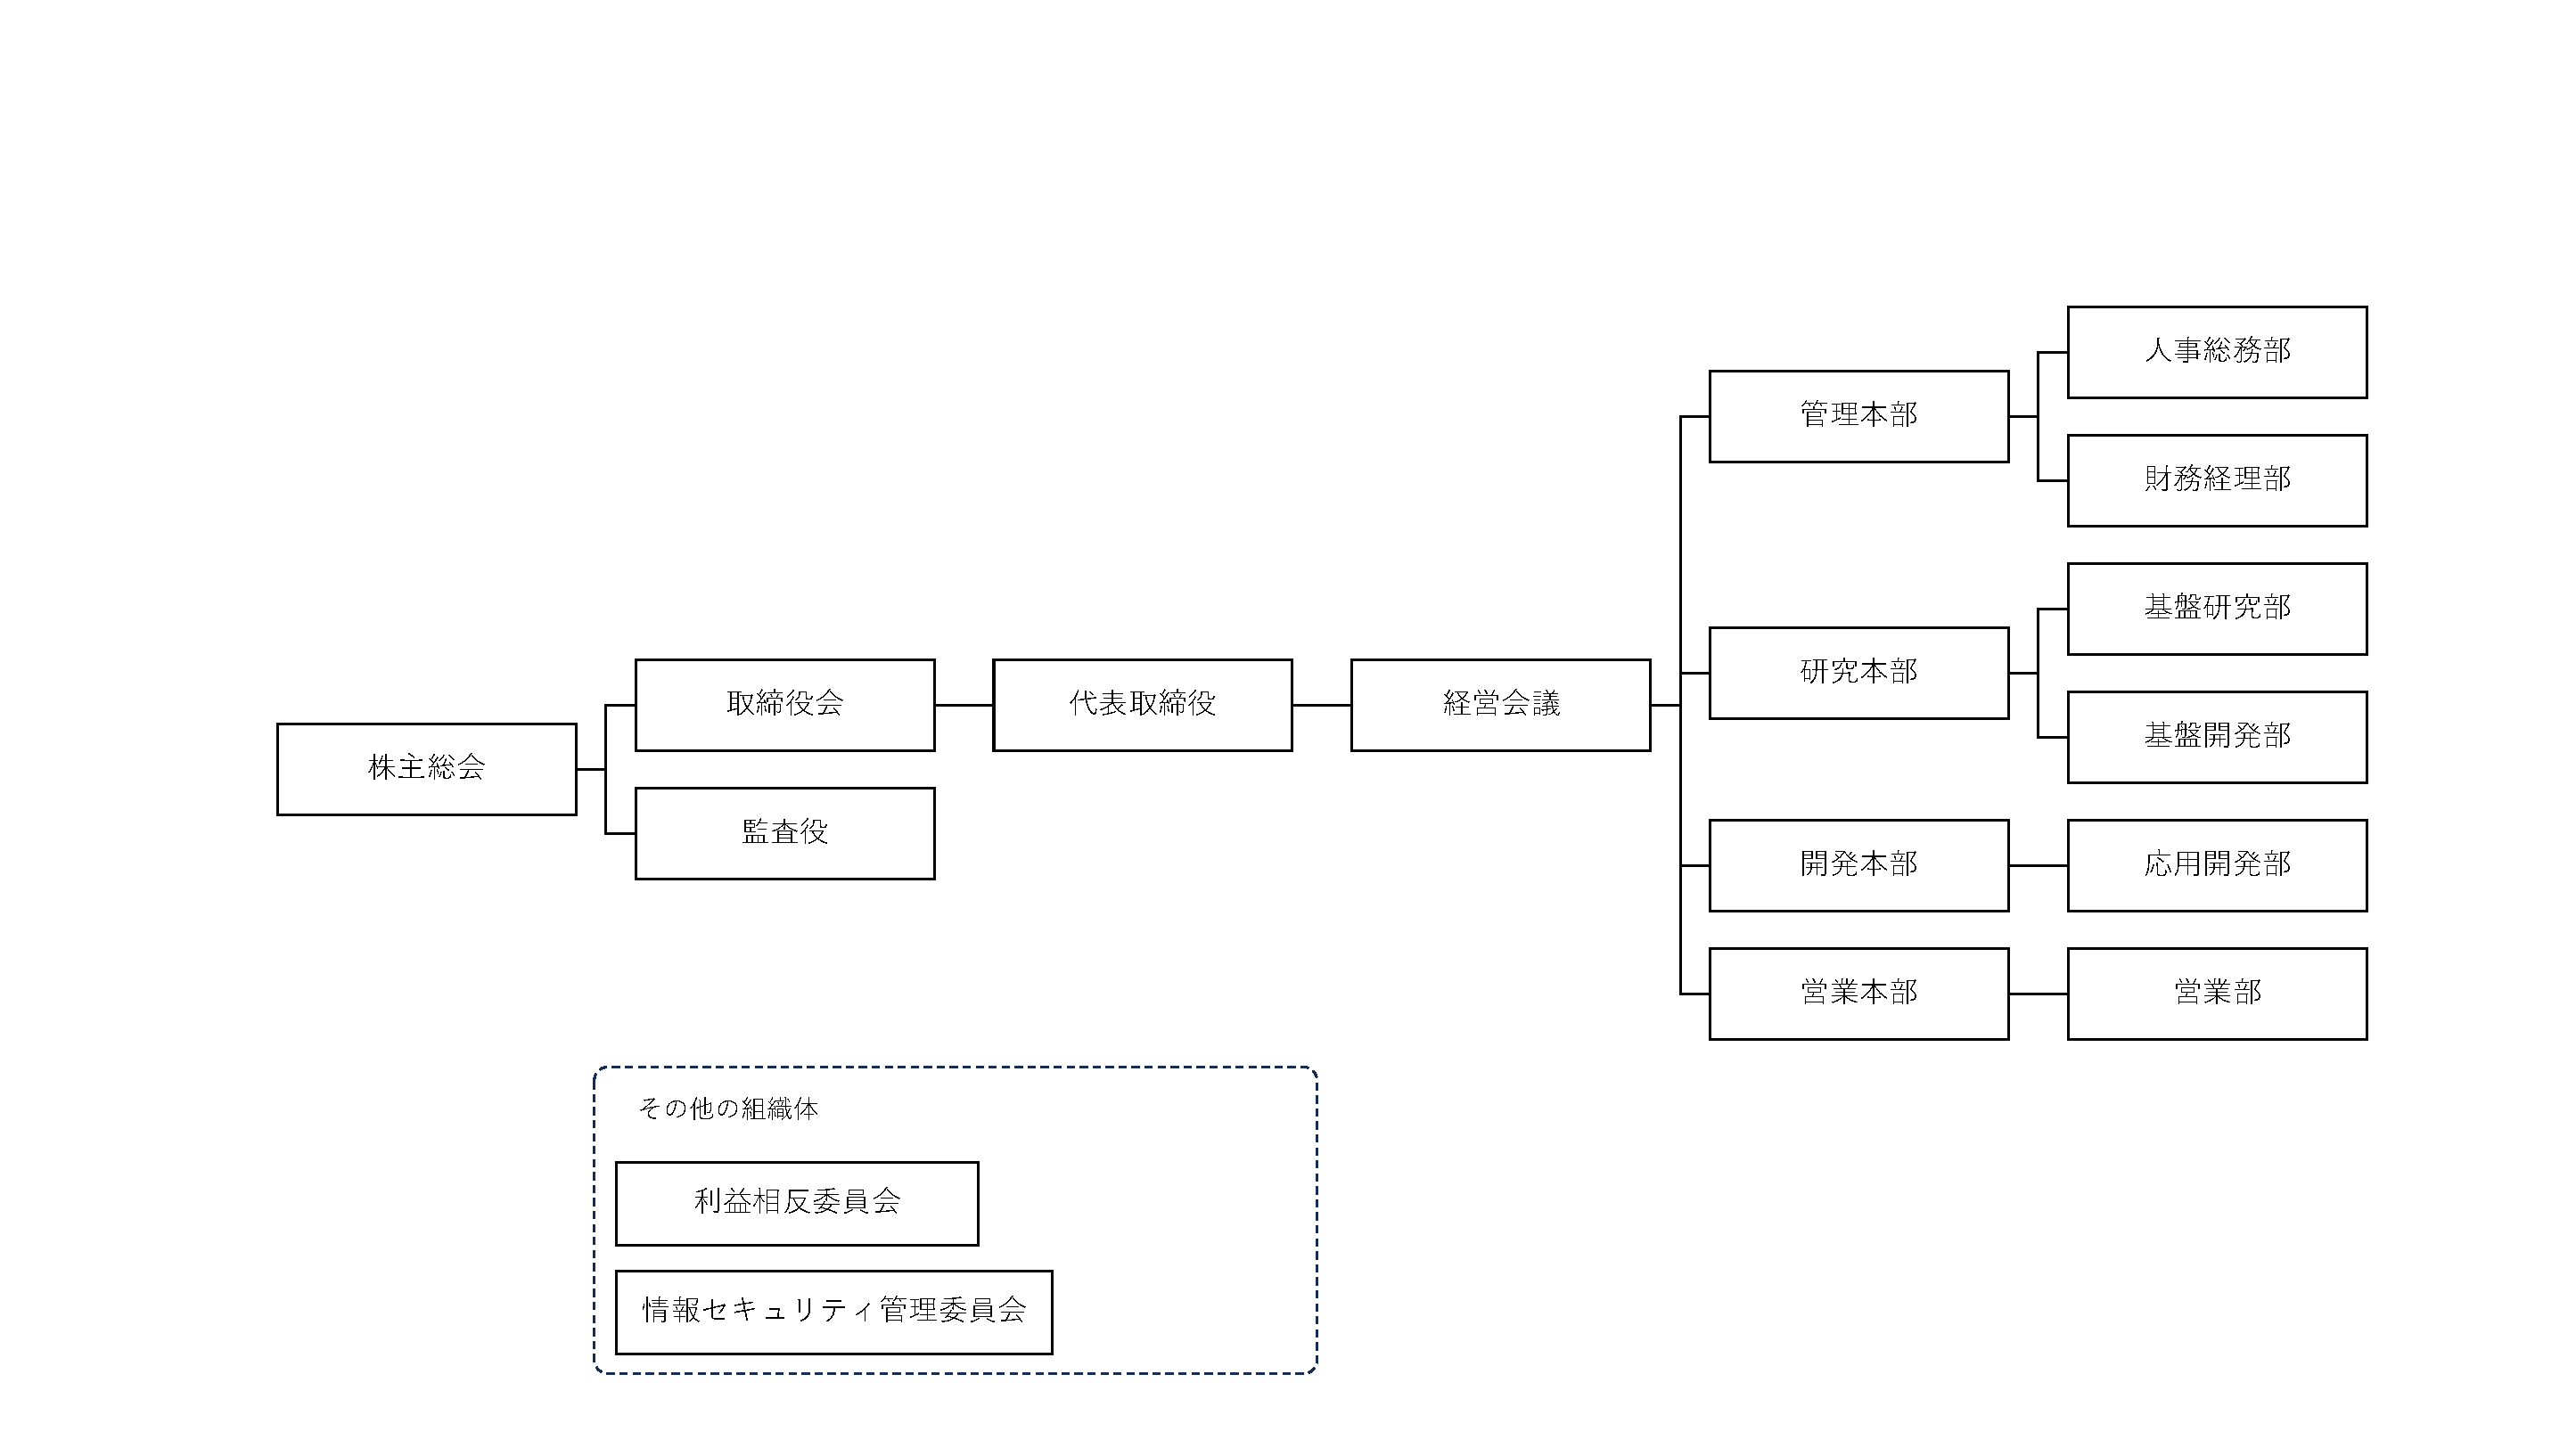
\includegraphics[trim={1cm 0cm 1cm 0cm},clip,width=1.0\linewidth]{soshiki.pdf}
\caption{当会社における組織図}
\end{figure}


\end{document}
